
\documentclass[10pt]{beamer}

\usetheme[progressbar=frametitle]{metropolis}
\usepackage{appendixnumberbeamer}

\usepackage{booktabs}
\usepackage[scale=2]{ccicons}

\usepackage{pgfplots}
\usepgfplotslibrary{dateplot}

\usepackage{caption}
\usepackage{subcaption}
\usepackage{subfigure}
\usepackage{subfig}


% QUOTES %
\usepackage[style=british]{csquotes}
\def\signed #1{{\leavevmode\unskip\nobreak\hfil\penalty50\hskip1em
  \hbox{}\nobreak\hfill #1%
  \parfillskip=0pt \finalhyphendemerits=0 \endgraf}}

\newsavebox\mybox
\newenvironment{aquote}[1]
  {\savebox\mybox{#1}\begin{quote}\openautoquote\hspace*{-.7ex}}
  {\unskip\closeautoquote\vspace*{1mm}\signed{\usebox\mybox}\end{quote}}


\usepackage{xspace}
\newcommand{\themename}{\textbf{\textsc{metropolis}}\xspace}

\newcommand*{\mytitle}{On Savings Optimisation Strategies}
\newcommand*{\myauthor}{Alejandro Jiménez Rico}
\newcommand*{\mysupervisor}{Isabel Serra \& Montserrat Guillén}
\newcommand*{\mytutor}{Isabel Serra}
\newcommand*{\myuni}{Centre de Recerca  Matemàtica}
\newcommand*{\mydate}{July 2018}

\title{
  \mytitle \\
}

\author{
  \emph{\myauthor} \\[2.0cm]
  \small \textbf{Academic tutor}: \mytutor \\
  \small \textbf{Supervised by}: \mysupervisor \\
}

\date{
  \mydate \\
}
% \titlegraphic{\hfill\includegraphics[height=1.5cm]{logo.pdf}}

\begin{document}

\maketitle

\begin{frame}{Outline}
  \setbeamertemplate{section in toc}[sections numbered]
  \tableofcontents[hideallsubsections]
\end{frame}

\section{On Risk Measures}

\begin{frame}[fragile]{Final Wealth distribution}
  \begin{figure}[h]
    \centering
    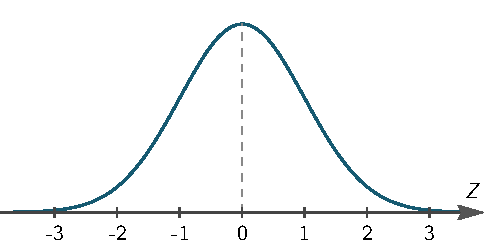
\includegraphics[scale=1]{none.pdf}
    \caption{Theoretical normal distribution.}
    \label{fig:volatility}
  \end{figure}
\end{frame}

\begin{frame}[fragile]{Volatility}

  \begin{figure}[h]
    \centering
    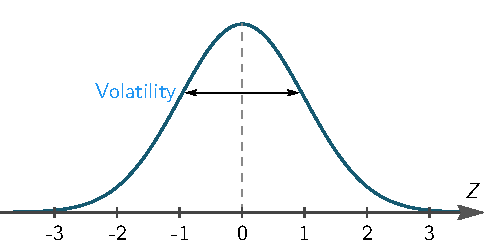
\includegraphics[scale=1]{volatility.pdf}
    \caption{Volatility as measure for dispersion or risk.}
    \label{fig:volatility}
\end{figure}
\end{frame}

\begin{frame}[fragile]{Value at Risk (VaR)}
  \begin{figure}[h]
    \centering
    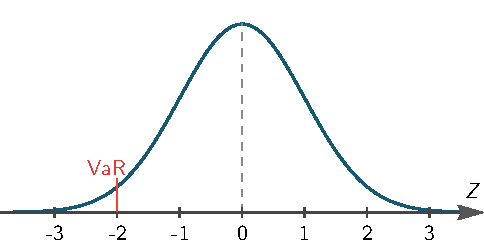
\includegraphics[scale=1]{var.pdf}
    \caption{Value ar Risk (VaR) is the quantile 5\%.}
    \label{fig:var}
  \end{figure}
\end{frame}

\begin{frame}[fragile]{Expected Shortfall}

  \begin{figure}[h]
    \centering
    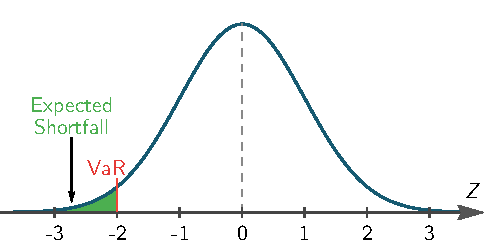
\includegraphics[scale=1]{es.pdf}
    \caption{Expected Shortfall is the average of the beyond-the-VaR distribution.}
    \label{fig:es}
\end{figure}
\end{frame}

\section{Optimising Investment Strategies}

\begin{frame}[fragile]{Constant Proportion Portfolio
Insurance (CPPI)}
  \begin{equation*}
    X_{t+1} = \qty(1 + N(\alpha, \sigma))X_t \pi + \qty(1 - \pi)X_t + C_t
  \end{equation*}

  \begin{figure}[h]
    \centering
    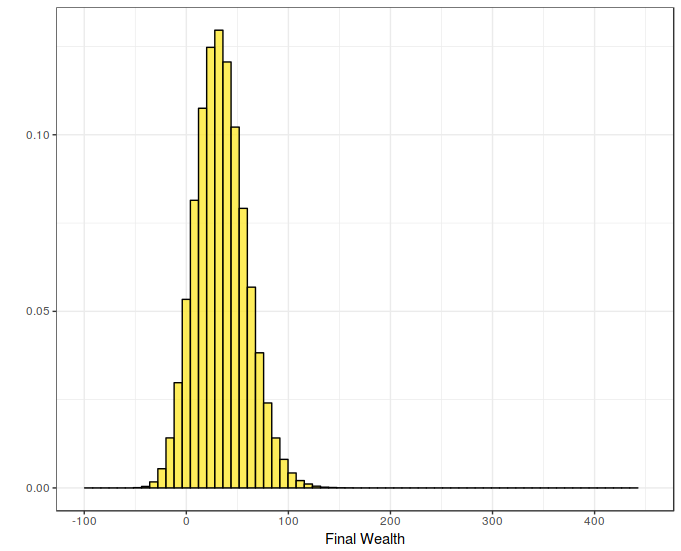
\includegraphics[scale=0.3]{fw_cppi.png}
    \caption{Results of the simulation for the CPPI model. Final wealth obtained for every simulation, over $100,000$ simulations, where $T=60$, $\mu = 0.0343$, $\sigma = 0.1544$, $a=10$, $\pi = 0.1$.}
    \label{fig:fw_cppi}
\end{figure}
\end{frame}

\begin{frame}[fragile]{Alternative}
  \begin{align*}
    \pi_t X_t &= A\qty(K + X_t + C_t) \\
    X_{t+1} &= \qty(1 + N(\alpha, \sigma))X_t \pi_t + \qty(1 - \pi_t)X_t + C_t
  \end{align*}

  \begin{figure}[h]
    \centering
    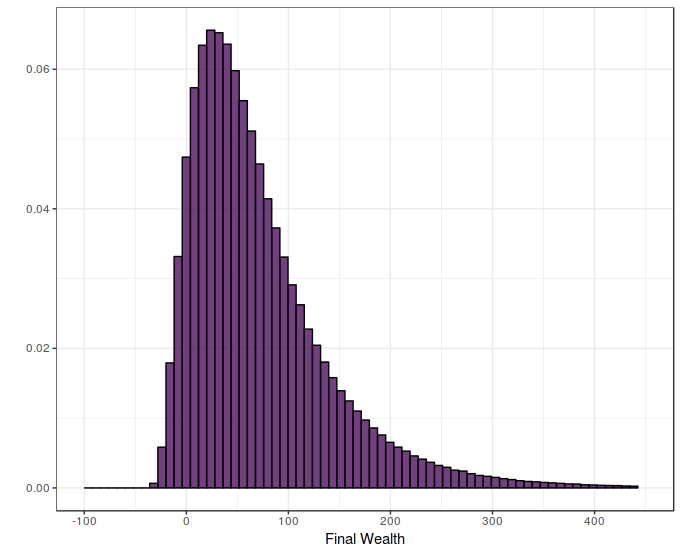
\includegraphics[scale=0.3]{fw_alt.png}
    \caption{Results of $100,000$ simulations for the \textit{Alternative} model. Final wealth obtained for every simulation, where $T=30$, $\mu = 0.0343$, $\sigma = 0.1544$, $a=10$, $\pi = 0.1$.}
    \label{fig:fw_alt}
  \end{figure}
\end{frame}

\begin{frame}[fragile]{Comparison}
  \begin{figure}[htbp]
    \centering
    \subfloat[Whole distribution of the Final Wealth for both strategies.\label{fig:1a}]{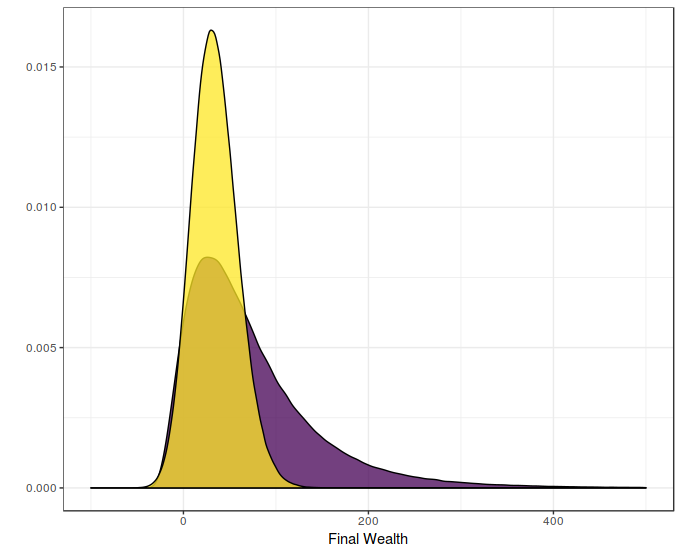
\includegraphics[width=0.5\textwidth]{fw_both.png}}\hfill
    \subfloat[Losses obtained from both strategies.\label{fig:1b}] {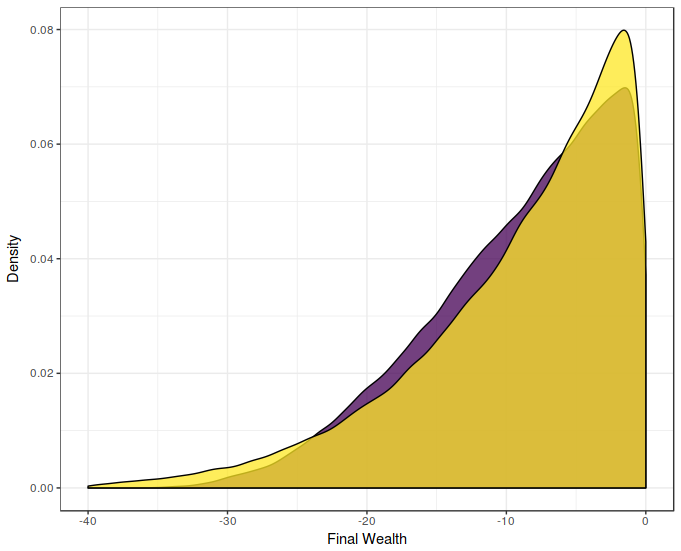
\includegraphics[width=0.5\textwidth]{loss_both.png}}
    \caption{Results of the simulation for the both strategies. Final wealth obtained for every simulation. The yellow one is the CPPI, and the purple one is the Alternative. Results from over $100,000$ simulations for each strategy, using $\alpha = 0.343$, $\sigma = 0.1544$, $a = 10$, $T = 60$, $A = 0.5$, $\pi = 0.1$, $K = 42$.} \label{fig:1}
  \end{figure}
\end{frame}

\begin{frame}[fragile]{Comparison}
  \begin{table}[h]
    \centering
    \caption{Results of $100,000$ simulations using different risk levels, with $\alpha = 0.343$, $\sigma = 0.1544$, $a = 10$, $T = 60$, $A = 0.5$ and therefore $ES/K = -3.3$. These results match approximately those presented in \cite{a:guillen-optimisation}, on Table 1 at page 8. Any differences are attributable to the intrinsic randomness of simulations.}
    \label{tab:cppi_alt}
    \begin{tabular}{ccccccc}
    \textbf{$\pi$} & \textbf{ES } & \textbf{$K$} & \textbf{CPPI ret} & \textbf{Alt ret} & \textbf{diff}  & \textbf{equiv $\pi$}\\
    0.1   & -12.47  & 40.59  & 0.33     & 0.51    & 0.18    & 0.17\\
    0.2   & -27.03  & 87.98  & 0.65     & 0.98    & 0.38    & 0.30 \\
    0.3   & -42.99  & 139.95 & 0.95     & 1.42    & 0.46    & 0.45 \\
    0.4   & -60.13  & 195.71 & 1.23     & 1.83    & 0.60    & 0.61 \\
    0.5   & -78.25  & 255.02 & 1.5      & 2.22    & 0.71    & 0.69 \\
    0.6   & -99.96  & 325.36 & 1.76     & 2.63    & 0.87    & 0.92 \\
    0.7   & -120.61 & 392.56 & 2.00     & 3.00    & 1.00    & * \\
    0.8   & -144.71 & 471.02 & 2.23     & 3.40    & 1.17    & * \\
    0.9   & -172.94 & 562.92 & 2.39     & 3.81    & 1.42    & * \\
    1     & -205.09 & 667.57 & 2.58     & 4.27    & 1.70    & *
  \end{tabular}
\end{table}
\end{frame}

\begin{frame}[fragile]{Comparison of Expected Shortfalls}
  \begin{figure}[h]
    \centering
    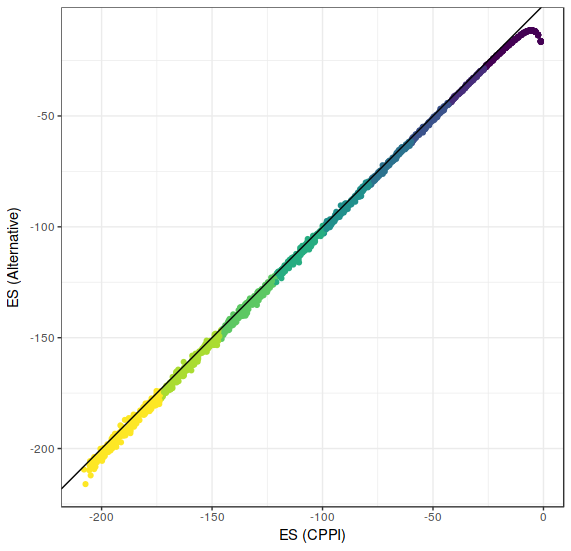
\includegraphics[scale=0.35]{es-es_pi.png}
    \caption{Plot that shows the relation between equivalent $\pi$ and $A$. Results from $20,000,000$ simulations performed for many different values of $\pi$ and $A$, with $\alpha = 0.343$, $\sigma = 0.1544$, $a = 10$, $T = 60$.}
    \label{fig:es}
  \end{figure}
\end{frame}

\begin{frame}[fragile]{Comparison}
  \begin{figure}[h]
    \centering
    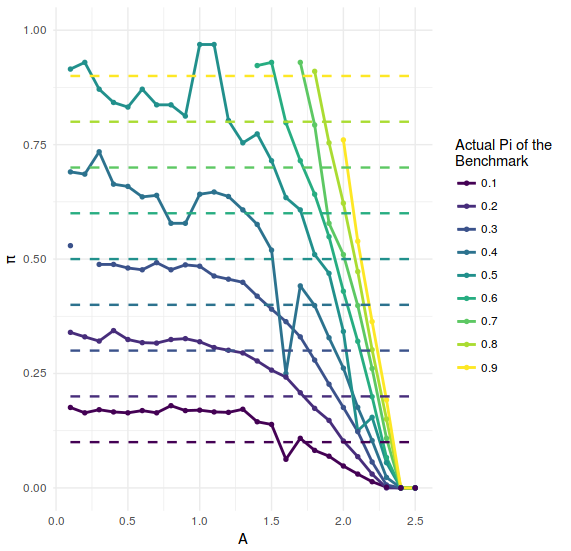
\includegraphics[scale=0.35]{pi-A-all-pis.png}
    \caption{Plot that shows the relation between equivalent $\pi$ and $A$. Results from $20,000,000$ simulations performed for many different values of $\pi$ and $A$, with $\alpha = 0.343$, $\sigma = 0.1544$, $a = 10$, $T = 60$.}
    \label{fig:es}
  \end{figure}
\end{frame}

\section{Pooled Funds}

\begin{frame}[fragile]{Simulating Mortality}

The work of \cite{a:schmeiser-binomial} proved that, given a Binomial Distribution, where
  \begin{align*}
    Pr(X = k) = \frac{n!}{k!(n-k)!} p^k (1-p)^{n-k} \emph{,}
  \end{align*}
we can numerically generate $k$ given $p$ and $n$. (The algorithm to do so is packed in the base R library.)
\end{frame}

\begin{frame}[fragile]{Simulating Mortality}
  \begin{align*}
    M = \frac{k}{n}w
  \end{align*}

  \begin{align*}
    \pi_t X_t &= A\qty(K + X_t + C_t) \\
    X_{t+1} &= \qty(1 + N(\alpha, \sigma))X_t \pi_t + \qty(1 - \pi_t)X_t + C_t + M_tX_t
  \end{align*}
\end{frame}

\begin{frame}[fragile]{Comparing Strategies with Mortality}
    \begin{figure}[htbp]
    \centering
    \subfloat[first caption.\label{fig:1a}]{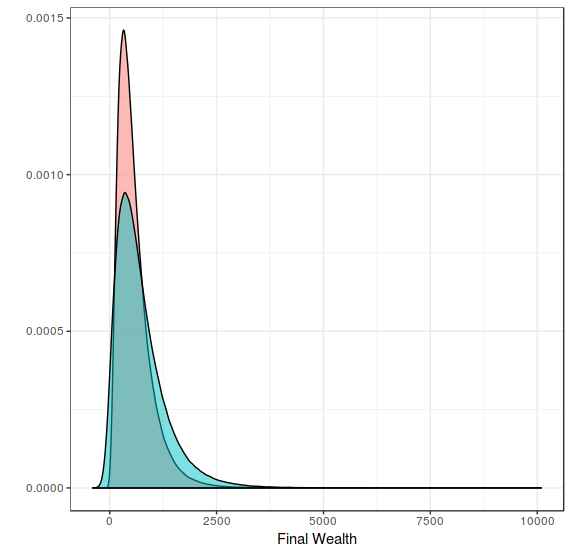
\includegraphics[width=0.5\textwidth]{mort_final_wealth.png}}\hfill
    \subfloat[second caption.\label{fig:1b}] {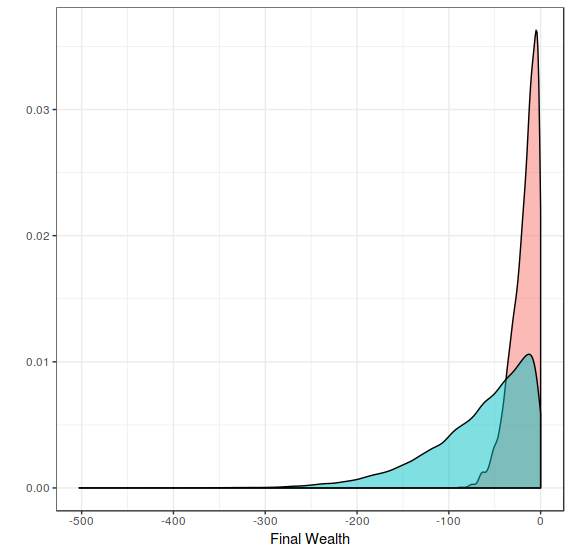
\includegraphics[width=0.5\textwidth]{loss_both_mort.png}}
    \caption{Results of the simulation for the both models with mortality. Final wealth obtained for every simulation. The blue one is the CPPI, and the red one is the Alternative. Results from over $100,000$ simulations for each strategy, using $\alpha = 0.343$, $\sigma = 0.1544$, $a = 10$, $T = 60$, $A = 0.5$ and $\pi = 0.1$.} \label{fig:1}
  \end{figure}
\end{frame}

\begin{frame}[fragile]{Comparing Strategies with Mortality}
  \begin{table}[h]
    \centering
    \caption{Results of $100,000$ simulations of both CPPI and Alternative models in a Pooled Fund, using different risk levels, with $\alpha = 0.343$, $\sigma = 0.1544$, $a = 10$, $T = 60$, $A = 0.5$ and $w = 1$.}
    \label{tab:cppi_alt_mort}
    \begin{tabular}{ccccccc}
    \textbf{$\pi$} & \textbf{ES } & \textbf{$K$} & \textbf{CPPI ret} & \textbf{Alt ret} & \textbf{diff}  & \textbf{equiv $\pi$}\\
    10  & 140.32  & 18.11 & 1.84 & 1.97 & 0.13 & 0.15 \\
    20  & 88.75  & 88.41 & 2.13 & 2.79 & 0.65 & 0.34 \\
    30  & 58.50  & 96.45 & 2.66 & 2.80 & 0.13 & 0.32 \\
    40  & 20.85  & 165.75  & 3.13 & 3.59 & 0.46 & 0.49 \\
    50  & -28.11 & 232.00  & 3.46 & 4.17 & 0.70 & 0.64 \\
    60  & -73.18 & 294.04 & 3.83 & 4.67 & 0.83 & 1.06 \\
    70  & -118.58 & 381.23 & 4.24 & 5.40 & 1.15 & 1.63 \\
    80  & -153.69 & 424.03 & 4.77 & 5.85  & 1.07 & *                 \\
    90  & -223.58 & 524.09 & 4.88 & 6.77 & 1.88 & *                 \\
    100 & -261.12   & 618.38 & 5.16 & 6.79 & 1.62 & *

  \end{tabular}
\end{table}
\end{frame}

\begin{frame}[fragile]{Comparison of Expected Shortfalls}
  \begin{figure}[h]
    \centering
    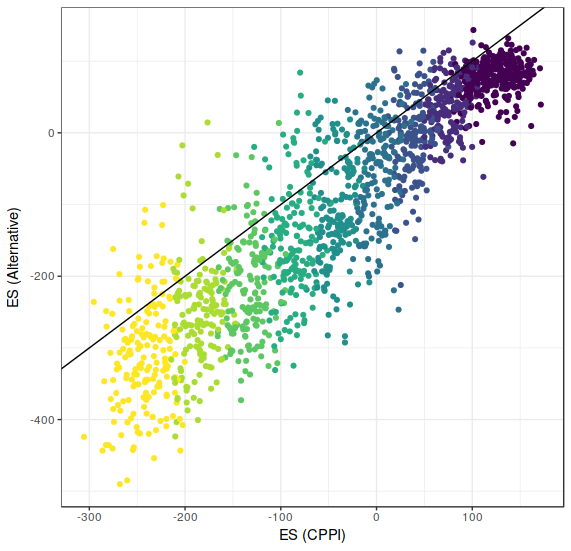
\includegraphics[scale=0.35]{es-es_mort_new.png}
    \caption{Plot that shows the relation between equivalent $\pi$ and $A$. Results from $20,000,000$ simulations performed for many different values of $\pi$ and $A$, with $\alpha = 0.343$, $\sigma = 0.1544$, $a = 10$, $T = 60$.}
    \label{fig:es}
  \end{figure}
\end{frame}

\begin{frame}[fragile]{Comparison}
  \begin{figure}[h]
    \centering
    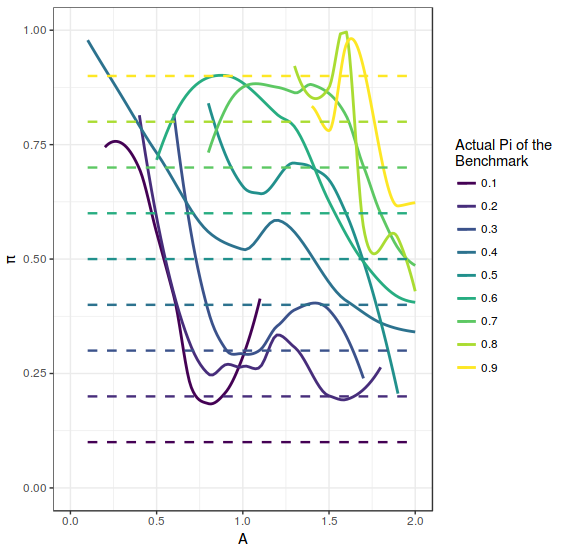
\includegraphics[scale=0.35]{pi-a_mort2.png}
    \caption{Plot that shows the relation between equivalent $\pi$ and $A$. Results from $20,000,000$ simulations performed for many different values of $\pi$ and $A$, with $\alpha = 0.343$, $\sigma = 0.1544$, $a = 10$, $T = 60$.}
    \label{fig:es}
  \end{figure}
\end{frame}

\section{Tails Analysis as Risk Assessment}

\begin{frame}[fragile]{What is a Tail?}
  \begin{align*}
    Z = \qty(Y-u | Y>u)
  \end{align*}
    \begin{figure}[h]
    \centering
    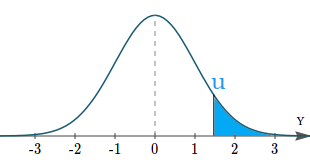
\includegraphics[scale=0.65]{tail.png}
    \caption{The value $u$ from which the Tail begins is not well defined, and os is up to every case to set it.}
    \label{fig:var}
  \end{figure}
\end{frame}


\begin{frame}[fragile]{General Pareto Distribution (GPD)}


The Pickands-Balkema-de Haan theorem states that for a large class of distributions $Z$,
exists $u$ such as that $F_u$ is well approximated by the Generalized Pareto Distribution
(GPD), whose standard cumulative distribution function is:
\[F_{\xi}(y) = \left\{
  \begin{array}{lr}
    1 - \qty(1 + \xi \frac{y}{\psi})^{\sfrac{-1}{\xi}} & : \xi \neq 0\\
    1 - e^{-\frac{y}{\psi}} & : \xi = 0
  \end{array}

  \begin{itemize}
    \item $\xi > 0$. The tail does not converge to zero, ever. Power-lawl
    \item $\xi = 0$. The tail converges to zero at infinity. Exponential.
    \item $\xi < 0$. The tail sharply converges to zero in a finite point.
\end{itemize}

\right. \emph{.}
\]
\end{frame}

\begin{frame}[fragile]{Coherent Risk Measures}
  \begin{align}
    \begin{split}
        \rho(\lambda X) &= \lambda \rho (X) \\
        \rho(\lambda  + X) &= \lambda + \rho(X) \\
        P(X_1 < X_2) &= 1 \implies \rho(X_1) < \rho(X_2) \\
        \rho(X_1 + X_2) &\leq \rho(X_1) + \rho(X_2) \emph{.}
    \end{split}
  \end{align}
\end{frame}

\begin{frame}[fragile]{Scale and Location free Risk Measures}
  \begin{align}
    \begin{split}
        \rho(\lambda X) &= \rho(X) \\
        \rho(\lambda + X) &= \rho(X) \\
        P(X_1 < X_2) &= 1 \implies \rho(X_1) < \rho(X_2) \\
        \rho(X_1 + X_2) &\leq \rho(X_1) + \rho(X_2) \emph{.}
    \end{split}
  \end{align}
\end{frame}

\begin{frame}[fragile]{Fitting a GPD}
  \begin{figure}[h]
    \centering
    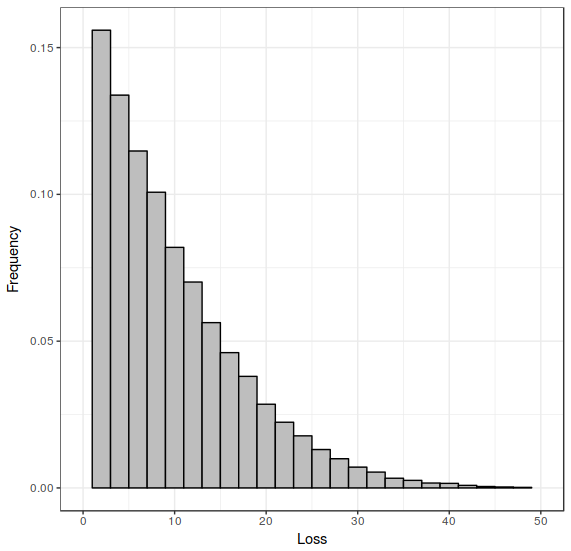
\includegraphics[scale=0.45]{cppi-losses-hist.png}
    \caption{Frequency Histogram of the losses of the CPPI strategy. Using $\pi = 0.1$, $T=60$, $\alpha = 0.0343$, $\sigma = 0.1544$, $a=10$ and $1,000,000$ simulations.}
    \label{fig:cppi-losses-histogram}
  \end{figure}
\end{frame}

\begin{frame}[fragile]{Fitting a GPD}
  \begin{figure}[h]
    \centering
    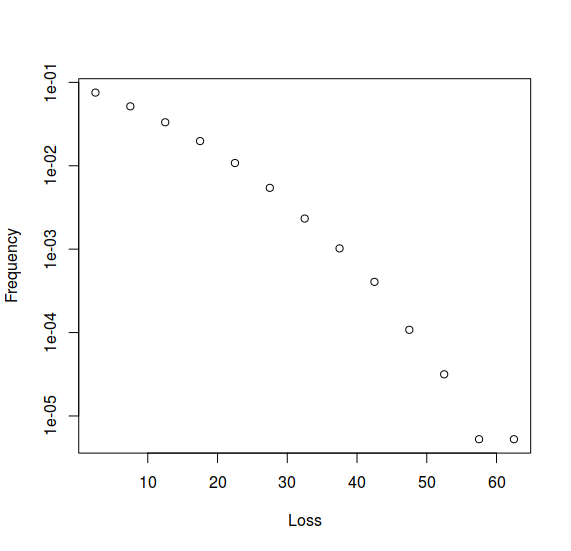
\includegraphics[scale=0.45]{cppi-dens-points.png}
    \caption{Density Distribution of the losses of the CPPI strategy in a logarithmic scale. Using $\pi = 0.1$, $T=60$, $\alpha = 0.0343$, $\sigma = 0.1544$, $a=10$ and $1,000,000$ simulations.}
    \label{fig:cppi-dens-points}
  \end{figure}
\end{frame}

\begin{frame}[fragile]{Fitting a GPD}
  \begin{figure}[h]
    \centering
    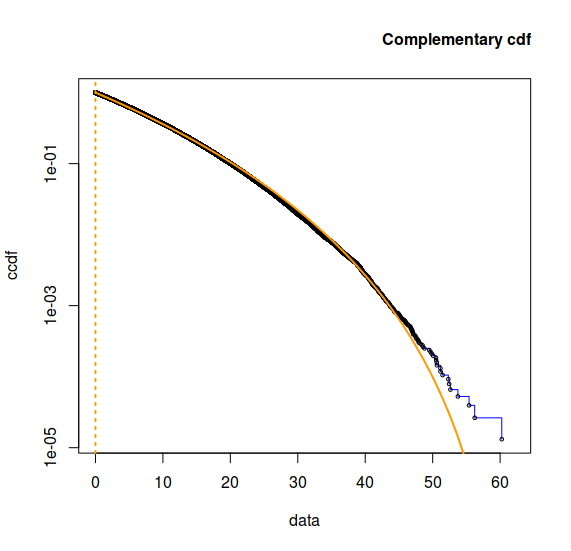
\includegraphics[scale=0.45]{cppi-ccdf-0.png}
    \caption{Fitted GPD using $u = 0 $ as a threshold. Using $\pi = 0.1$, $T=60$, $\alpha = 0.0343$, $\sigma = 0.1544$, $a=10$ and $1,000,000$ simulations.}
    \label{fig:cppi-ccdf-0}
  \end{figure}
\end{frame}

\begin{frame}[fragile]{Fitting a GPD}
  \begin{figure}[h]
    \centering
    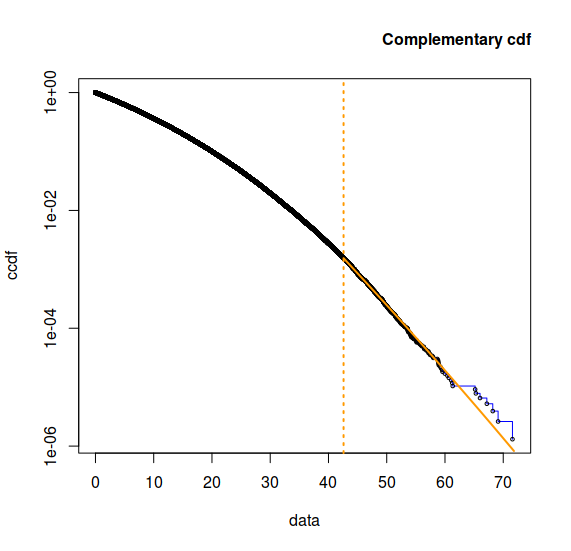
\includegraphics[scale=0.4]{cppi-ccdf-autothresh.png}
    \caption{Fitted GPD using Using $\pi = 0.1$, $T=60$, $\alpha = 0.0343$, $\sigma = 0.1544$, $a=10$ and $1,000,000$ simulations. \\

    Turned out to be $u = 42.59$ and $\xi = 0.14$}
    \label{fig:cppi-ccdf-autothresh}
  \end{figure}
\end{frame}

\begin{frame}[fragile]{Extreme Value Index (EVI) $\xi$}
  \begin{figure}[h]
    \centering
    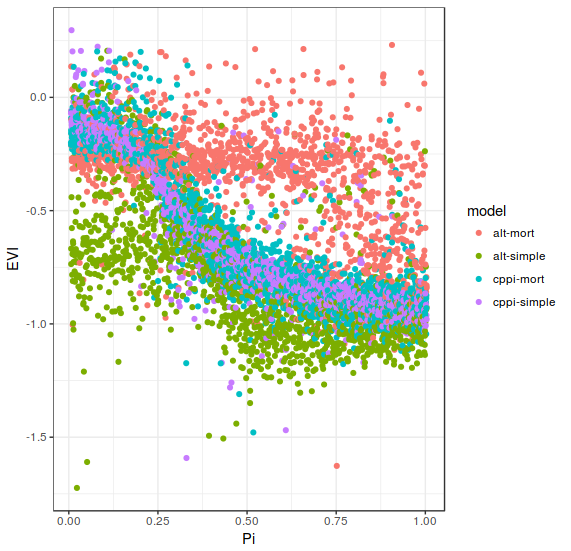
\includegraphics[scale=0.45]{evi-pi_new.png}
    \caption{Extreme Value Index measured by varying values of $\pi$ and $A$.  Using $\alpha = 0.0343$, $\sigma = 0.1544$, and $1000000$ simulations.}
    \label{fig:evi-pi}
  \end{figure}
\end{frame}

\begin{frame}[fragile]{Extreme Value Index (EVI) $\xi$}
  \begin{figure}[h]
    \centering
    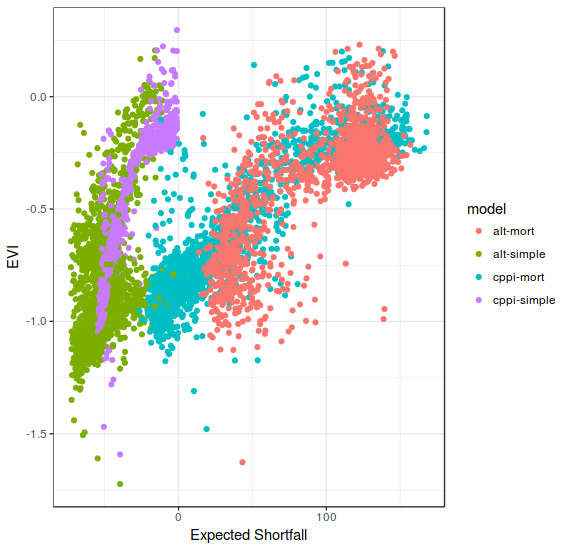
\includegraphics[scale=0.45]{evi-es_new2.png}
    \caption{Extreme Value Index vs Expected Shortfall. Scatter plot of $10,000,000$ simulations of all four strategies, iterating over all values of $0 <= \pi <= 1$ and $0.1 <= A <= 2$.}
    \label{fig:evi-es}
  \end{figure}
\end{frame}

\section{Conclusion}

\begin{frame}[fragile]{Summary}
  \begin{itemize}
    \item It is optimal to define a $K$ value in order to set the risk level of the investor.
    \item Pooled Funds can dramatically increase the return of savings strategies without compromising the risk aversion levels.
    \item Parameters that define the shape of losses tails can serve as location and scale free risk measures.
  \end{itemize}
\end{frame}

\begin{frame}{}
  \begin{aquote}{Adam Smith}
    All money is a matter of belief.
  \end{aquote}
\end{frame}

{\setbeamercolor{palette primary}{fg=black, bg=yellow}
\begin{frame}[standout]
  Questions?
\end{frame}
}

\appendix

\begin{frame}[allowframebreaks]{References}
  \bibliographystyle{ieeetr}
  \bibliography{bibliography.bib}
\end{frame}

\end{document}
